% !TeX root = ../main.tex
% Add the above to each chapter to make compiling the PDF easier in some editors.

\begin{figure}[t!]
    \centering
    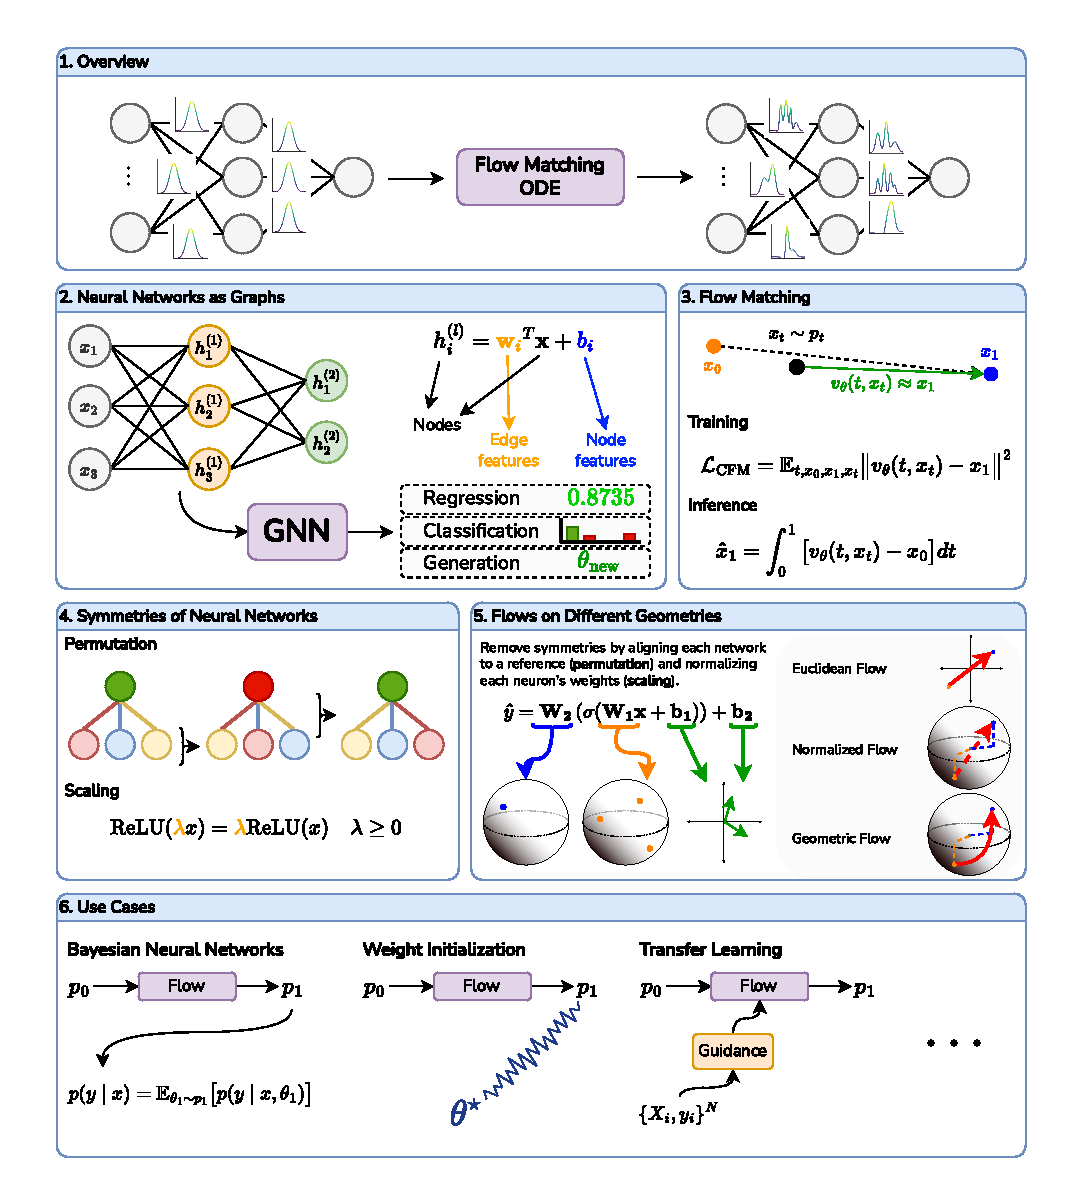
\includegraphics[width=\linewidth]{figures/weightflow.drawio.pdf}
    \caption{\label{fig:main}\textbf{Overview of our weight-space flow.} We aim to learn a flow in weight-space \textit{(1)}, processing neural networks with GNNs \textit{(2)}, using flow matching \textit{(3)} and taking into account the symmetries of neural network weights \textit{(4)}. We propose three different flows \textit{(5)} and potential use cases include Bayesian neural networks, learned weight initialization, or transfer learning \textit{(6)}.}
\end{figure}

\chapter{Introduction}\label{chapter:introduction}

Deep generative models such as diffusion and flow models that have led to significant developments in image generation \citep{esserScalingRectifiedFlow2024b} or biological applications such as protein structure prediction \citep{abramsonAccurateStructurePrediction2024} have also been applied to neural network weights \citep{peeblesLearningLearnGenerative2022,schurholtHyperRepresentationsLearningPopulations2024a}. However, the existing works do not take into account the geometry of neural networks arising from the permutation and scaling symmetries of neural networks. We attempt to fill this gap by building flow models that learn a vector field to transport a prior over neural network to the posterior for a specific task through the flow matching framework \citep{lipmanFlowMatchingGuide2024}, processing neural network weights with permutation-invariant graph neural networks \citep{kofinasGraphNeuralNetworks2024,limGraphMetanetworksProcessing2023} and propose three candidate designs differing on how they handle the underlying geometry. Figure \ref{fig:main} gives an overview of our approach, and we summarize the main points in this Introduction. 

\subsubsection{Symmetries of Neural Networks (Chapter \ref{section:geometry_of_nns})}

Neural networks are subject to various symmetries, transformations of the network parameters that leave the function unchanged, which have been an active research area since the early days of neural network research \citep{hecht-nielsenALGEBRAICSTRUCTUREFEEDFORWARD1990}. For instance, permuting the neurons in one layer together with the outgoing weights in an MLP preserves the function, as well as similarly permuting the channels in a convolutional neural network. Non-linear activation functions induce further scaling symmetries \citep{godfreySymmetriesDeepLearning2022}; e.g. for a constant $\lambda \geq 0$, $\text{ReLU}(\lambda x) = \lambda \text{ReLU}(x)$. In addition to these static symmetries, other forms of symmetries might arise from the structure of the data, or dynamically during phases of training {\color{red} [cite here?]}. 

Accounting for these symmetries in a weight-space learning task by using architectures with the correct inductive biases, through data augmentation \citep{shamsianImprovedGeneralizationWeight2024} or by removing the symmetries by mapping neural networks to canonical representations \citep{pittorinoDeepNetworksToroids2022} can reduce the effective dimensionality of the problem and make weight-space learning better scalable.  

\subsubsection{Neural Networks as Graphs (Chapter \ref{section:wsl})}

A neural network can naturally be modeled as a graph, and this has fueled a recent line of work building graph neural networks (GNNs) that take as input other neural networks \citep{kofinasGraphNeuralNetworks2024,limGraphMetanetworksProcessing2023,kalogeropoulosScaleEquivariantGraph2024}. The nodes often correspond to the neurons in an MLP or channels in a convolutional network and the edges to the weights. Used with the appropriate positional encodings, this graph formalism provides an effective way of handling the permutation symmetries of various kinds of neural networks, and has also been extended to account for scaling symmetries as well \citep{kalogeropoulosScaleEquivariantGraph2024}. Since a GNN is not restricted to graphs with a certain structure, weight-space GNNs have the additional benefit that the same GNN can be used to process different neural networks, even those with different architectures altogether.

In building our flows, we also process neural networks using GNNs, mode specifically the Relational Transformer model \citep{diaoRelationalAttentionGeneralizing2023} that incorporates an attention mechanism with edge updates. 

\subsubsection{Generative Modeling with Flow Matching (Chapter \ref{section:flow_models})}

Flow matching (FM) \citep{lipmanFlowMatchingGenerative2023,albergoStochasticInterpolantsUnifying2023,liuFlowStraightFast2022,tongImprovingGeneralizingFlowbased2023} generalizes diffusion models with a more flexible framework and a simple simulation-free regression objective. Given two sampleable marginal distributions $p_0$ and $p_1$, a coupling $(x_0, x_1)$ is sampled from a joint distribution, and $x_t$ from the conditional intermediate distribution $p_t(x_t \mid x_0, x_1)$ with $t$ sampled within the interval $[0,1]$. A neural network (velocity model) is then trained to predict the conditional velocity $u_t(x_t \mid x_0, x_1)$; e.g. $x_1 - x_0$. Marginalizing over the joint coupling then results in a time-dependent vector field that transforms $p_0$ to $p_1$, which is estimated by solving a differential equation with the velocity given by the trained velocity model. 

We train our models using flow matching as well, with a Gaussian prior and the posterior samples collected through the neural networks' optimization trajectories, experimenting with different couplings. Our slightly modified flow matching training setup is described in more detail in Section \ref{sec:fm_training}.

\subsubsection{Flows with Different Geometries (Chapter \ref{chapter:method})}

We consider ReLU MLPs, and to remove the permutation symmetries, we align all neural networks to the same reference network using the rebasin operation \citep{ainsworthGitReBasinMerging2023,penaReBasinImplicitSinkhorn2023} that permutes a neuron's weights to minimize the loss barrier between two networks. To handle the scaling symmetries, we build on the canonicalization procedure of \citep{pittorinoDeepNetworksToroids2022}, where each neuron's incoming weights are normalized and its outgoing weights are inversely scaled to preserve the function being computed; the last layer is further normalized globally in classification networks. This gives the neural network a product geometry, with the bias vectors as Euclidean vectors, intermediate neurons on the hypersphere, and the last layer (optionally) on the hypersphere as a whole. 

We then compare three different kinds of flows: first a Euclidean flow that ignores the scaling symmetries, then a Normalized flow with the weights embedded in the product geometry but with the velocity field defined in Euclidean space (i.e. inside the hyperspheres), and finally a fully Geomtric flow with the flow with the velocity field defined on the product geometry as well using the Riemannian Flow Matching framework \citep{chenRiemannianFlowMatching2023}. 

\subsubsection{Overview of Results (Chapter \ref{chapter:results})}

We evaluate our flows on a variety of tasks after training them on samples obtained with gradient-based optimization methods and show that for small networks on relatively easier tasks, they can directly generate weights matching or sometimes exceeding the performance of optimized weights. On more complex tasks and larger models, while direct generation does not match the quality of optimized weights, Bayesian model averaging over a number of samples leads to comparable predictive performance. Finally we show that the weights generated from a flow trained on weights from one task can be transferred to different tasks, either by using them as learned weight initializations, or by guiding the sampling process with task gradients. {\color{red} SCALING results}



\section{Reproducibility and Guide to Code}


